\setchapterpreamble[u]{\margintoc}
\chapter{Searching and Sorting}
\labch{searchandsorting}
In this chapter are introduced the most important and used algorithms about \textbf{searching}, which retrieve some data stored in a particular data structure \cite{wikisearch} (\href{https://en.wikipedia.org/wiki/Search_algorithm}{Search algorithm, Wikipedia}), and \textbf{sorting}, which put in a certain order some data stored in a list \cite{wikisorting} (\href{https://en.wikipedia.org/wiki/Sorting_algorithm}{Sorting algorithm, Wikipedia}).
\section{Binary Search}
Let us consider the problem of finding a number stored in an array with an \textbf{ascending} order (Figure \ref{sorting_1}).

\begin{figure}[hb]
	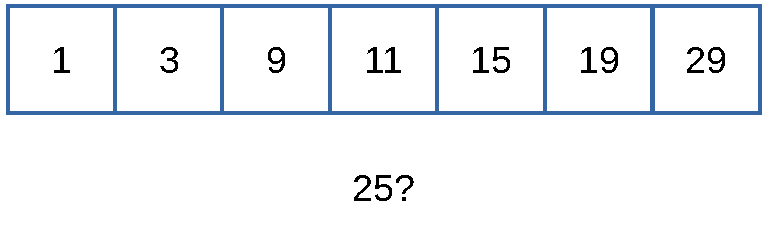
\includegraphics[width=11cm,height=4.5cm]{chapters/searchandsorting/images/sorting_1.pdf}
	\caption[]{An array with numeric values ordered in an ascending order.}
	\labfig{sorting_1}
	\label{sorting_1}
\end{figure}

A first way to tackle the problem could be to check all the numbers of the array, in others words this method consists in performing a loop all over the elements of the array and check one by one if the number where is the element we are looking for. The complexity of this method is \(O(n)\) because in the worst case we have to look at all the elements of the array. 

There is a more efficient way to search an element in an ascending ordered array then the method showed previously. This method is called \textbf{binary search} \cite{wikibinarysearch} (\href{https://en.wikipedia.org/wiki/Binary_search_algorithm}{Binary Search Algorithm, Wikipedia}).
Let us start to check as the first element the central value of the array (in case the array has an even number of elements there are two central values, and one can choose the bigger or the lower). If the central element is the one we are looking for the search ends, otherwise, because the array is ascending ordered, we can ignore one half of the array. If the central number is bigger than the number we are looking for thus we will ignore the right half of the array, if the central number is lower than the number we are looking for thus we will ignore the left half of the array. This procedure is repeated: we consider the central value of the new array, which has half of the size of the previous step, and we check is that value is the one we are looking for, and we repeat the procedure until or we find or we do not find the number we are looking for (Figure \ref{sorting_2}). 

\begin{figure}[hb]
	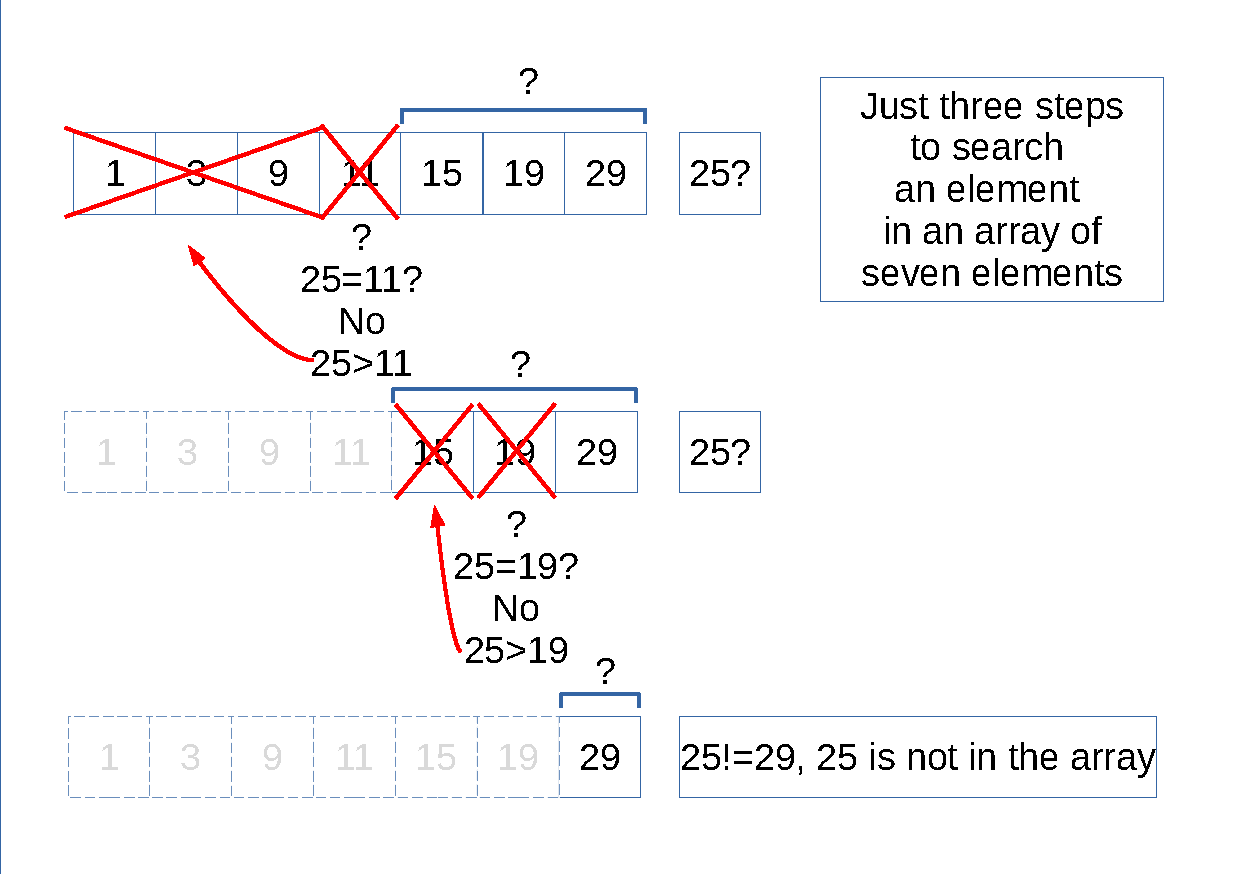
\includegraphics[width=14cm,height=6cm]{chapters/searchandsorting/images/sorting_2.pdf}
	\caption[]{Binary Search Algorithms steps.}
	\labfig{sorting_2}
	\label{sorting_2}
\end{figure}

\subsection{Efficiency of the Binary Search Algorithm}
For evaluating the efficiency of this algorithm we have to evaluate the number of steps required for solving the problem. We already know that the efficiency of this algorithm will not be \(O(n)\), because in this algorithm not all the elements of the array are checked. The way for evaluating the complexity of an algorithm is to execute the algorithms varying the size of the input, and evaluating how many operations are done in the worst case. In the binary search algorithm the worst case is when the size of the array becomes one, so we find or we do not find the searched element at the end of the array splitting process.

\begin{table}[h]
\caption[Binary Search Efficiency]{The number of iterations grows of one every power of two, in others words it grows as \(log(n)\).}
\labtab{binarysearchefficiency}
\begin{tabular}{ | l | c | c | c | c | c | c | c | c | c |}
   
    \multicolumn{1}{l}{} & \multicolumn{1}{c}{} & 
    \multicolumn{1}{c}{\(2^{0}\)} & \multicolumn{1}{c}{\(2^{1}\)} &
    \multicolumn{1}{c}{} & \multicolumn{1}{c}{\(2^{2}\)} & 
    \multicolumn{1}{c}{} & \multicolumn{1}{c}{}          & 
    \multicolumn{1}{c}{} & \multicolumn{1}{c}{\(2^{3}\)} \\
    \hline
	Array Size & 0 & \cellcolor{LightCyan} 1 & \cellcolor{LightCyan} 2 & 3 & \cellcolor{LightCyan} 4  & 5 & 6 & 7 & \cellcolor{LightCyan} 8 \\
    \hline
	Iterations (worst case) & 0 & \cellcolor{LightCyan} 1 & \cellcolor{LightCyan} 2 & 2 & \cellcolor{LightCyan} 3 & 3 & 3 & 3 & \cellcolor{LightCyan} 4 \\
	\hline	
\end{tabular}
\end{table}

We observe that the exponent of the power of two is the number of iteration minus one, or at the contrary the number of iteration is the exponent of a power plus one.
\begin{center}
\(log( power\ of\ exponent\ 2 + 1) = log_{2}(n) + 1\)
\end{center}
In general it is used \(log\) and is said that the binary search algorithm has a complexity of \(log(n)\). 

\newpage
\subsection{Binary Search Implementation}
The following code is the python implementation of the binary search algorithm.
\begin{lstlisting}[caption={Binary search python implementation.}]
def binary_search(array_input, value):
	low = 0
	high = len(array_input) - 1
	while low <= high:
		mid = (low + high) // 2
		if array_input[mid] == value:
			return mid
		elif value > array_input[mid]:
			new_low = mid + 1
		else:
			new_high = mid - 1
	return -1
\end{lstlisting}

\begin{figure}[hb]
	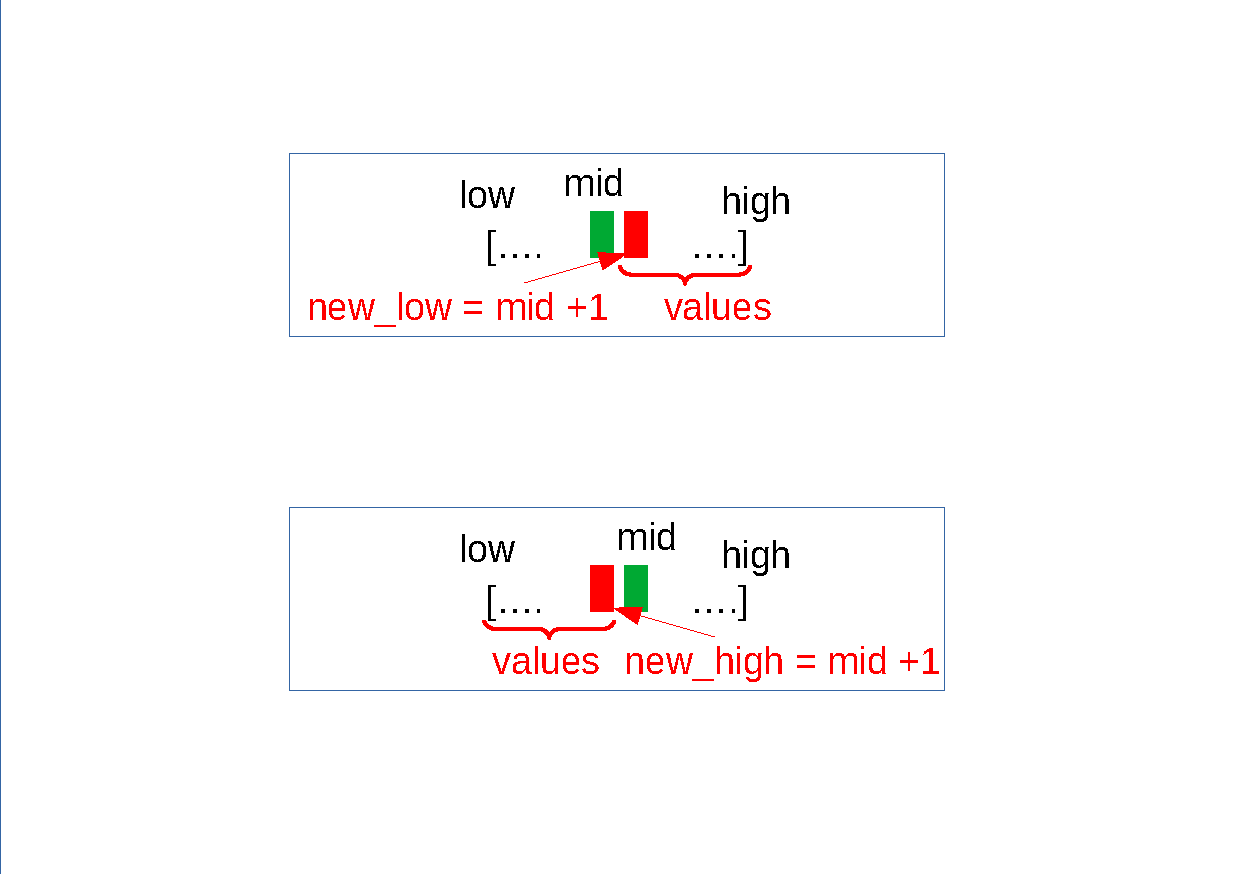
\includegraphics[width=14cm,height=6cm]{chapters/searchandsorting/images/sorting_3.pdf}
	\caption[]{Array splitting in the implementation of the binary search algorithm.}
	\labfig{sorting_3}
	\label{sorting_3}
\end{figure}

\newpage
\section{Bubble Sort}
\textbf{bubble sort} is the easiest sorting algorithm working on arrays. Bubble sort works by swapping two element at each step if they are in the wrong order, repeating this process until all the array is not completely ordered \cite{wikibubblesort} (\href{https://en.wikipedia.org/wiki/Bubble_sort}{Bubble Sort, Wikipedia}). In this algorithm the bigger elements tend to move at the bottom of the array, like bubbles that move at the top of a water bottle.

\begin{figure}[hb]
	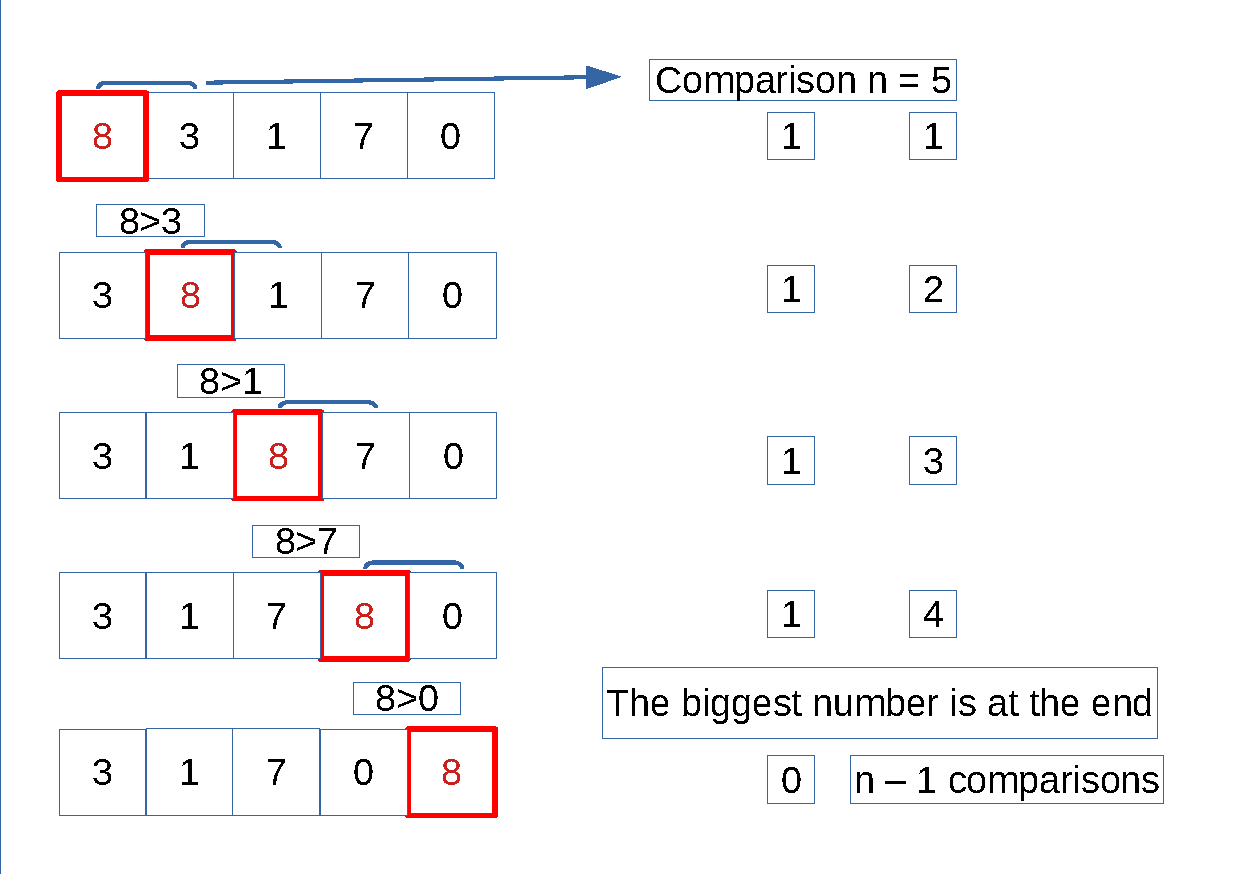
\includegraphics[width=14cm,height=6cm]{chapters/searchandsorting/images/sorting_4.pdf}
	\caption[]{Bubble sort algorithm. The biggest element goes at the and of the array.}
	\labfig{sorting_4}
	\label{sorting_4}
\end{figure}

\begin{figure}[hb]
	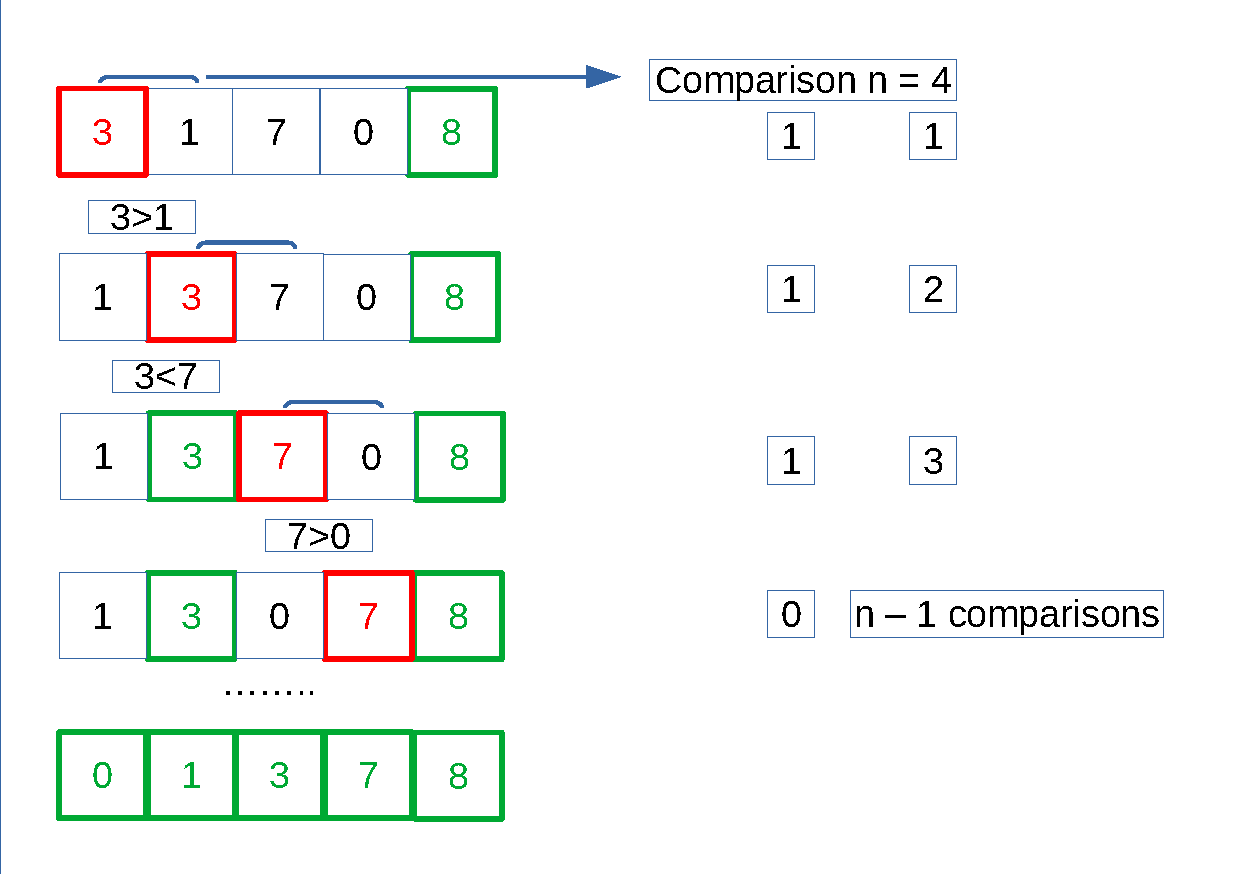
\includegraphics[width=14cm,height=6cm]{chapters/searchandsorting/images/sorting_5.pdf}
	\caption[]{The swapping process is repeated until the array is completely ordered.}
	\labfig{sorting_5}
	\label{sorting_5}
\end{figure}

\subsection{Efficiency of the Bubble Sort Algorithm}
For ordering an array using the bubble sort \(n - 1\) iterations are required, every step. The number of total steps are \(n - 1\), thus the total number of operations to be executed for ordering an array is \((n - 1)*(n - 1) = n^{2} - 2n + 1 = O(n^{2})\).
In summary:
\begin{itemize}
\item \textbf{Worst Case}: \(O(n^{2})\)
\item \textbf{Average Case}: \(O(n^{2})\)
\item \textbf{Best Case}: \(O(n)\). The array is already completely ordered and it is enough to cycle all the elements.
\end{itemize} 

\subsection{Bubble Sort Implementation}
The following code is the python implementation of the bubble sort algorithm.
\begin{lstlisting}[caption={Bubble Sort python implementation}]
def bubble_sort(array_input):
	index = len(array_input) - 1
	sorted = False
	
	while not sorted:
		sorted = True
		for i in range(0, index):
			if array_input[i] > array_input[i + 1]:
				sorted = False
				array_input[i], array_input[i + 1] = array_input[i + 1], array_input[i]
	return array_input
\end{lstlisting}

\section{Merge Sort}
The \textbf{merge sort} algorithm works by dividing the array in single elements at first, grouping and ordering all the elements two by two. After the first step we will have a lot of subarrays of two elements. The next step is to merge all these subarrays and to order the elements. The merging and ordering process is repeated until the array is unified again \cite{wikimergesort} (\href{https://en.wikipedia.org/wiki/Merge_sort}{Merge Sort, Wikipedia}).  This way of reducing a big problem in several smaller is called \textbf{Divide et impera} (Divide and conquer).

\begin{figure}[hb]
	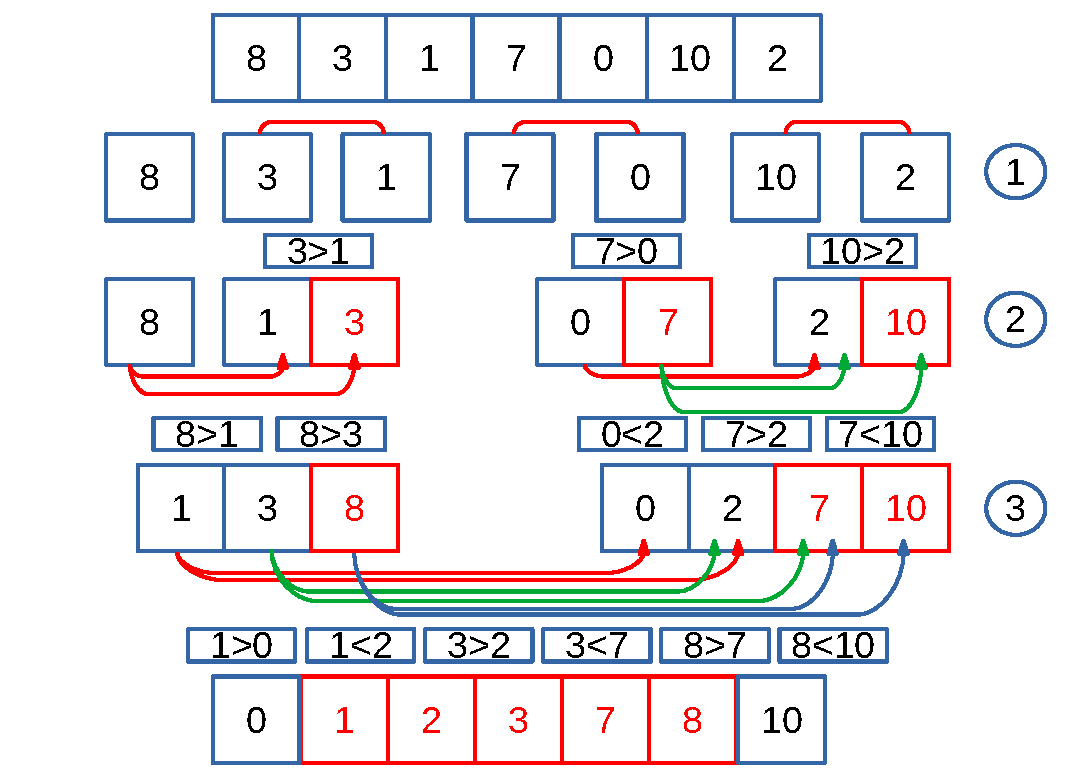
\includegraphics[width=14cm,height=6cm]{chapters/searchandsorting/images/sorting_6.pdf}
	\caption[]{Merge sort algorithm. The merging and sorting process is repeated until the array is again unified with all the elements sorted.}
	\labfig{sorting_6}
	\label{sorting_6}
\end{figure}

The steps are (Figure \ref{sorting_6}): 
\begin{itemize}
\item[1] Divide the array in subarryas of one element. Merge two by two and order the elements. The number of the subarrays is odd, so one array at this step is not merged. \textbf{The number of comparison for this step is 3}.
\item[2] Merge and order again the new subarrays. For ordering in this case we start from the first element of the array on the left, and we compare this value with all the elements of the array on the right. If the first element is bigger than the picked one from the array on the right is moved, otherwise is not moved and we go to the next element. \textbf{The number of comparison for this step is 5.}   
\item[3] Merge and order again as at the previous step. \textbf{The number of comparison for this step is 6.}
\end{itemize}

\subsection{Efficiency of the Merge Sort Algorithm}
For evaluating the efficiency of this algorithms we have to count the number of iterations and comparisons are being done. By using the example showed in Figure \ref{sorting_6} we will try to extrapolate a general pattern for an array of dimension \(n\).

The number of comparisons depends by the array size. For an array of two elements the number of comparisons is one, for one of three elements are two, for one of four are three, and for one of seven are six. It is impossible to calculate in general the number of comparisons, but it is possible to calculate the worst case given the array dimension. From the previous example we see that for each step the maximum number of comparisons is seven, the size of the array. The reason is that the sum of all subarrays is seven. In general the sum of all subarrays is always the size of the array. Thus the total efficiency is \(O(\# \ of\ comparison \ * \ \# \ of \ iterations \ )\).

How many iterations are required? In our example for an array of seven elements, the iterations required are three. From the subprocess of our example we observe that for an array of size four the number of iterations are two, for one of size three are two, and for one of size two is one. Thus we can create the following table:

\begin{table}[h]
\caption[Merge Sort Efficiency]{The number of iterations grows of one every power of two, in others words it grows as \(log(n)\).}
\labtab{mergesortefficiency}
\begin{tabular}{ | l | c | c | c | c | c | c | c | c | c |}
   
    \multicolumn{1}{l}{} & \multicolumn{1}{c}{\(2^{0}\)} & 
    \multicolumn{1}{c}{\(2^{1}\)} & \multicolumn{1}{c}{} &
    \multicolumn{1}{c}{\(2^{2}\)} & \multicolumn{1}{c}{} & 
    \multicolumn{1}{c}{} & \multicolumn{1}{c}{}          & 
    \multicolumn{1}{c}{\(2^{3}\)} & \multicolumn{1}{c}{} \\
    \hline
	Array Size & \cellcolor{LightCyan} 1 & \cellcolor{LightCyan} 2 & 3 & \cellcolor{LightCyan} 4 & 5  & 6 & 7 & \cellcolor{LightCyan} 8 & 9 \\
    \hline
	Iterations (worst case) & \cellcolor{LightCyan} 0 & \cellcolor{LightCyan} 1 & 2 & \cellcolor{LightCyan} 2 & 3 & 3 & 3 & \cellcolor{LightCyan} 3 & 4 \\
	\hline	
\end{tabular}
\end{table}

In conclusion the efficiency if \(O(n \ log(n))\), which is better than \(O(n^{2})\) of the bubble sort. 

The memory efficiency in this case is bigger than the bubble sort algorithm. For the merge sort some subarrays (in the worst case are \(n\)) are used and they need to be stored in the memory.

\newpage
\subsection{Merge Sort Implementation}
The following code is the python implementation of the merge sort algorithm.
\begin{lstlisting}[caption={Merge Sort python implementation.}]
def merge_sort(array_input):
	
	if len(array_input) > 1:
		mid = len(array_input)//2
		left_side = array_input[:mid]
		right_side = array_input[mid:]
		
		merge_sort(left_side)
		merge_sort(right_side)
		
		i = 0 # Left side index
		j = 0 # Right side index
		k = 0 # Sorted array index
		
		while i < len(left_side) and j < len(right_side):
			if left_side[i] < right_side[j]:
				array_input[k] = left_side[i]
				i+= 1
			else:
				array_input[k] = right_side[j]
				j+= 1
			k+= 1
			
		# Adding all elements if some of 
        # them have been left behind 
        while i < len(left_side): 
        	array_input[k] = left_side[i] 
            i+= 1
            k+= 1
            
        while j < len(right_side): 
        	array_input[k] = right_side[j] 
            j+= 1
            k+= 1
			
	return array_input
\end{lstlisting}

\begin{figure}[hb]
	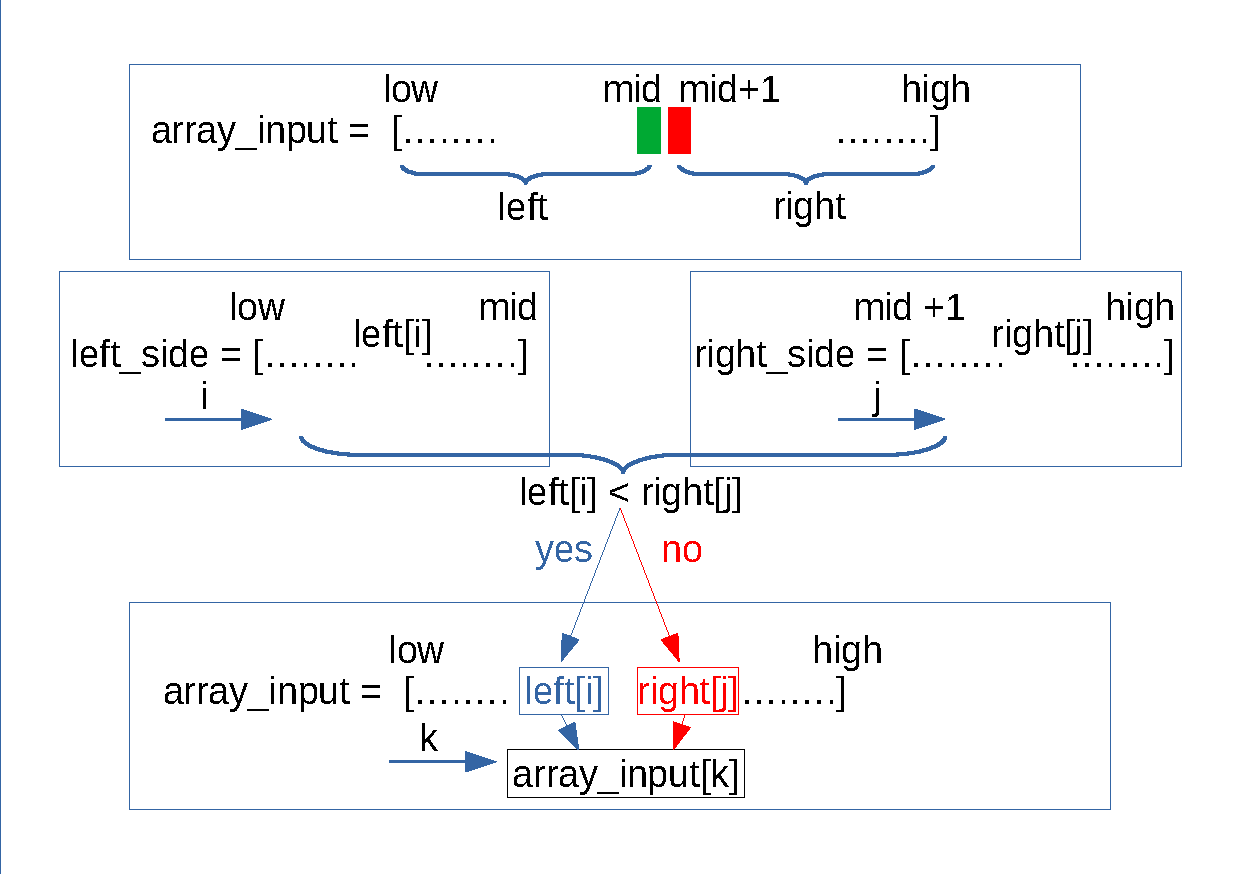
\includegraphics[width=14cm,height=6cm]{chapters/searchandsorting/images/sorting_7.pdf}
	\caption[]{Merge sort algorithm implementation.}
	\labfig{sorting_7}
	\label{sorting_7}
\end{figure}

\section{Quicksort}
The \textbf{quicksort} is a sorting algorithm of the divide et impera type. It works by randomly choosing an element of the array, called pivot, and putting all the bigger and lower values on its left or on its right respectively. This procedure is repeated recursively on the two new subarrays until all the elements have been a pivot \cite{wikiqicksort} (\href{https://en.wikipedia.org/wiki/Quicksort}{Qicksort, Wikipedia}). 
\begin{figure}[hb]
	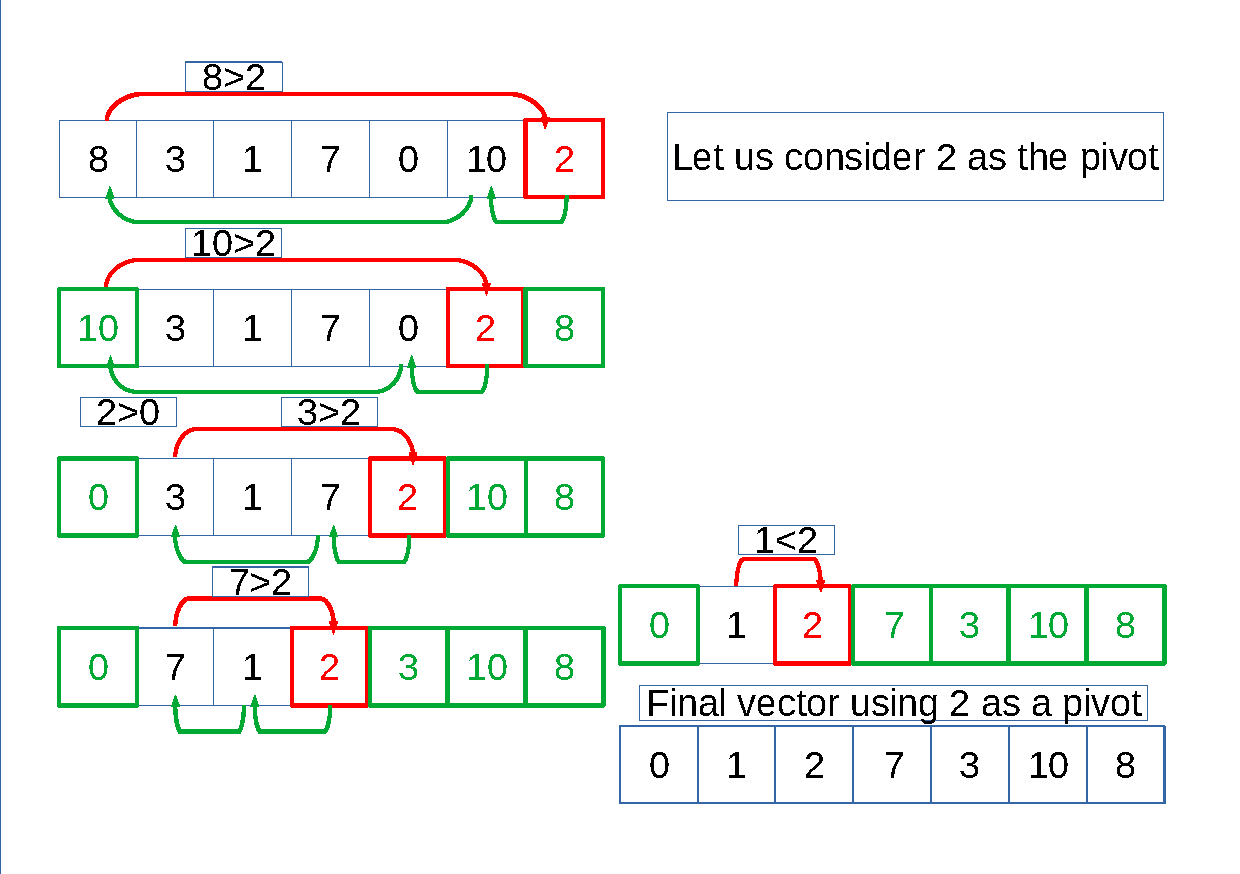
\includegraphics[width=14cm,height=6cm]{chapters/searchandsorting/images/sorting_8.pdf}
	\caption[]{Quicksort algorithm steps, part one.}
	\labfig{sorting_8}
	\label{sorting_8}
\end{figure}

\begin{figure}[hb]
	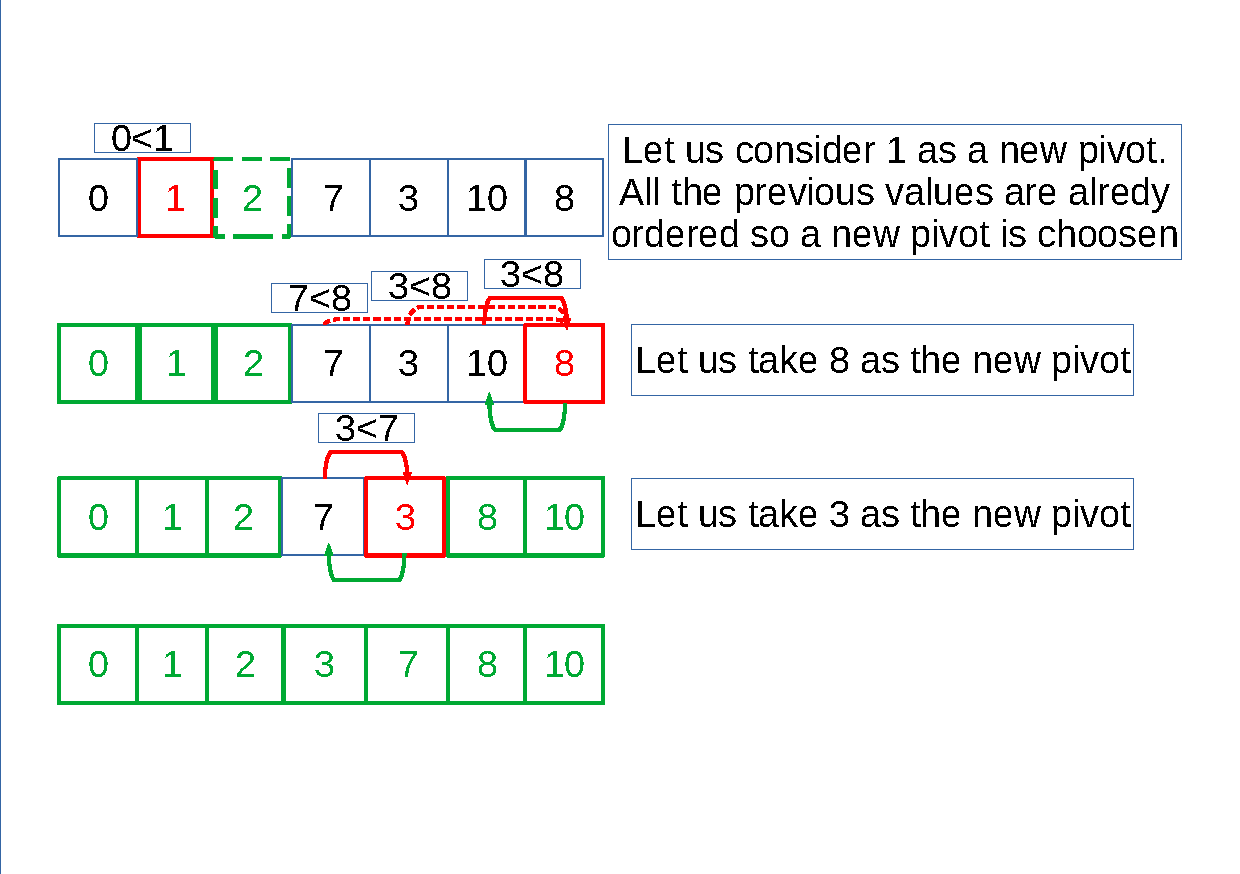
\includegraphics[width=14cm,height=6cm]{chapters/searchandsorting/images/sorting_9.pdf}
	\caption[]{Quicksort algorithm steps, part two.}
	\labfig{sorting_9}
	\label{sorting_9}
\end{figure}

Here are the steps of quicksort algorithm based on the example of Figure \ref{sorting_8} and Figure \ref{sorting_9}:
\begin{itemize}
\item[1] Let us consider the last element as pivot, two in this case, and let us compare it with all the elements to its left. Let us start from the first element of the array, and let us compare their values. In this case \(8 > 2\), so \(8\) is moved on the position of the pivot (\(2\)) which is moved of one position to the left. The number to be removed, \(10\) in this case, is moved in the first position.
\item[2] Let us repeat the process. Now we have to compare the pivot (\(2\)) in the new position with the first element (\(10\)), and because \(10>2\) we repeat the previous step of moving the elements.
\item[3] In this case \(0<2\) so we do not have to do anything, but going to the next element, \(3\) in this case.
\item[4] For the pivot \(2\) all the elements to the left are less than it, and all the element to the right are bigger than it. \(2\) is not moved anymore. We can change the pivot and repeat all the steps for the new pivots until all the elements have been a pivot.
\end{itemize}

\subsection{Efficiency of the Quicksort Algorithm}
Evaluating the efficiency of quicksort is very hard. In the following there are some justifications for the worst case, and for the best and average complexity.

Let us consider first the worst case. In this situation the last elements of the array are the bigger ones, so it is necessary to check all the previous elements, by doing \(n^{2}\) comparisons Figure \ref{sorting_10}.

\begin{figure}[hb]
	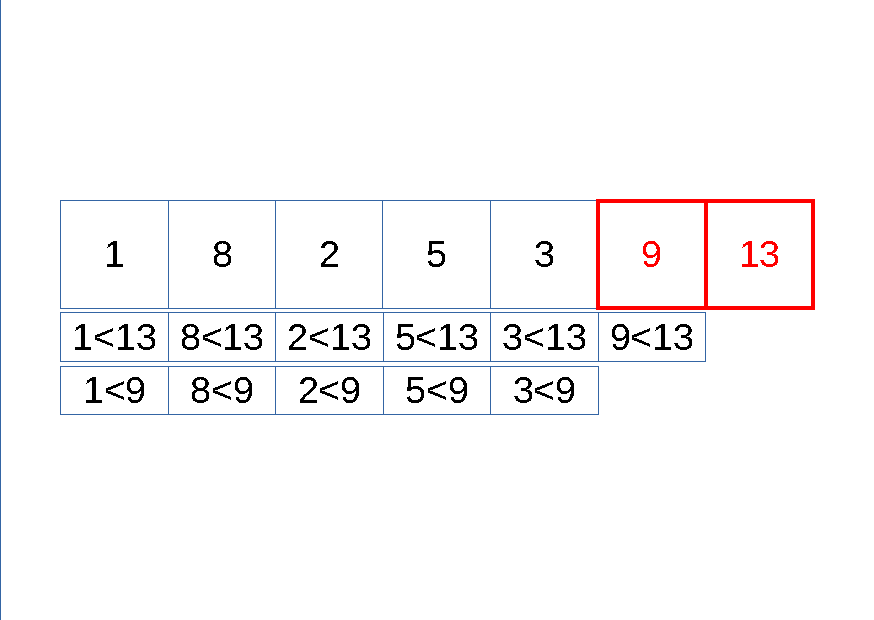
\includegraphics[width=14cm,height=6cm]{chapters/searchandsorting/images/sorting_10.pdf}
	\caption[]{Quicksort algorithm worst case.}
	\labfig{sorting_10}
	\label{sorting_10}
\end{figure}

In the best and in the average case the complexity is \(O(n log(n)\). The reason is because the first pivot tends to move at the center of the array, having in this way two subarrays. The pivots of these two subarrays will tend to move at their center and the process is repeated until all the elements have been a pivot, having in this way an ordered array.

\begin{figure}[hb]
	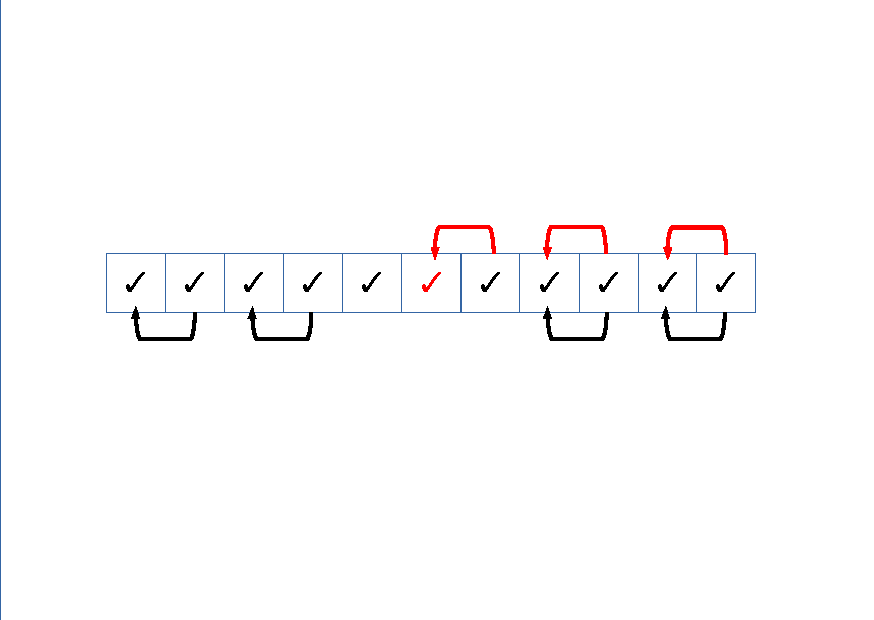
\includegraphics[width=14cm,height=6cm]{chapters/searchandsorting/images/sorting_11.pdf}
	\caption[]{Quicksort algorithm best and average case.}
	\labfig{sorting_11}
	\label{sorting_11}
\end{figure}

The space complexity of quicksort is constant, \(O(1)\).

This algorithm can be optimized in several ways. For example it is possible to order at the same time two half of the array, or considering as pivot always the last elements.

\paragraph{Quicksort and Merge Sort Comparison}
Quicksort is often a better solution than merge sort, because even if its worst case performance is \(O(n^{2})\), this problem can be solved by using the randomized quicksort. If the right pivot is chosen the problem related to having a worst case performance is solved. Moreover the quicksort algorithm dose not require an auxiliary memory, which is a big advance in a lot of situations.

On the other hand merge sort is a better solution than quicksort and heapsort \cite{wikiheapsort} (\href{https://en.wikipedia.org/wiki/Heapsort}{Heapsort, Wikipedia}) when the sorting is done on linked lists that do not require big auxilary space and on very large data sets stored on slow-to-access media, such as disk storage or network-attached storage \cite{wikiqicksort}.

\textbf{In summary}:
\begin{itemize}
\item \textbf{Worst Case}: \(O(n^{2})\)
\item \textbf{Average Case}: \(O(n\ log(n))\)
\item \textbf{Best Case}: \(O(n\ log(n))\)
\item \textbf{Space}: \(O(1)\)
\end{itemize}

\subsection{Quicksort Implementation}
The following code is the python implementation of the quicksort algorithm \cite{quicksortcode} (\href{https://www.educative.io/edpresso/how-to-implement-quicksort-in-python}{Quicksort Python Implementation}).
\begin{lstlisting}[caption={Quicksort python implementation.}]
def merge_sort(array_input):
	
	elements = len(array_input)
        
    # Base case
    if elements < 2:
    	return array_input
        
    # Position of the partitioning element
    current_position = 0

	# Partitioning loop
	for i in range(1, elements):
    	if array_input[i] <= array_input[0]:
        	current_position += 1
            temp = array_input[i]
            array_input[i] = array_input[current_position]
            array_input[current_position] = temp

    # Brings pivot to its appropriate position
    temp = array_input[0]
    array_input[0] = array_input[current_position]
    array_input[current_position] = temp
        
    # Sorts the elements to the left of pivot
    left = SortingAlgorithms.quicksort(array_input[0:current_position])
    # Sorts the elements to the right of pivot
    right = SortingAlgorithms.quicksort(array_input[current_position+1:elements])

    # Merging everything together
    array_input = left + [array_input[current_position]] + right

	return array_input
\end{lstlisting}

\begin{figure}[hb]
	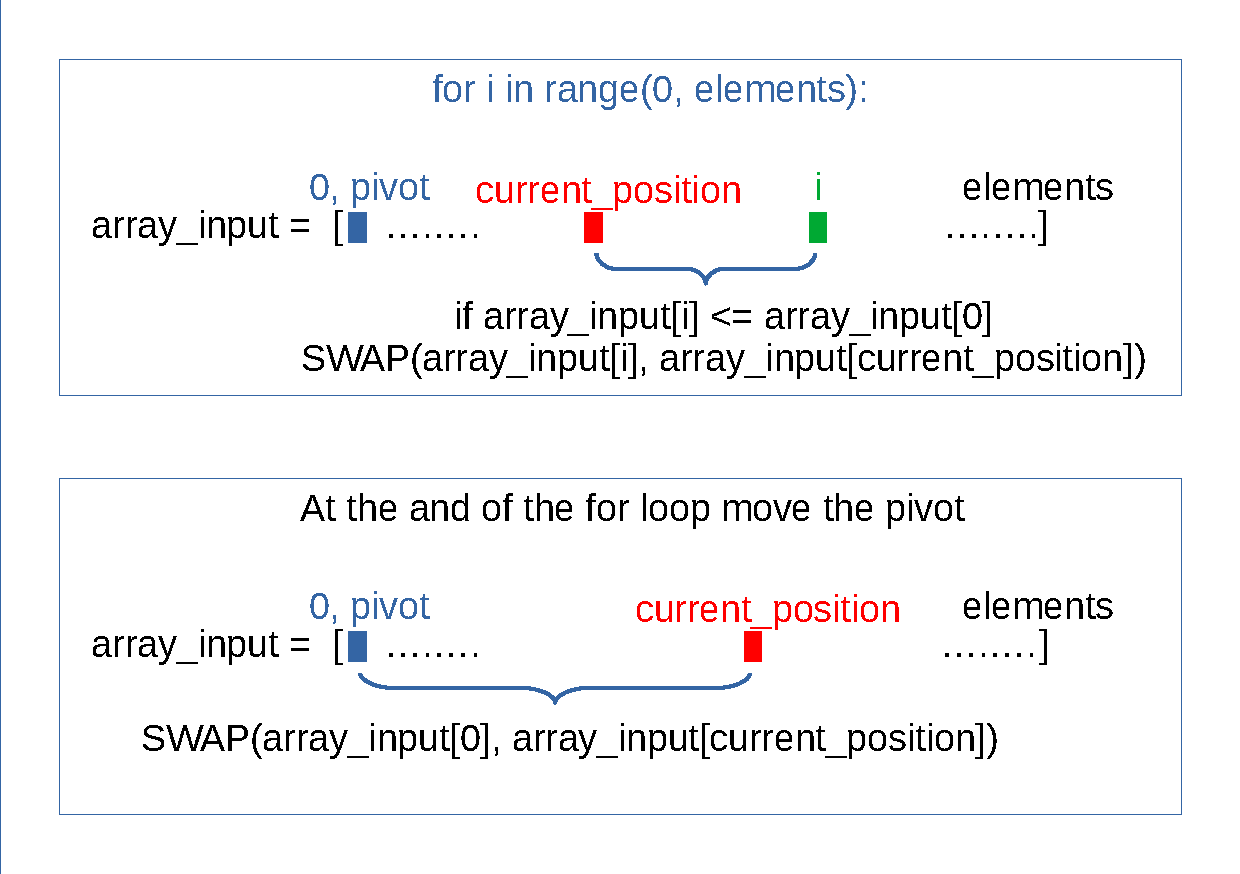
\includegraphics[width=14cm,height=6cm]{chapters/searchandsorting/images/sorting_12.pdf}
	\caption[]{Quicksort algorithm implementation.}
	\labfig{sorting_12}
	\label{sorting_12}
\end{figure}